%!TEX root = thesis.tex
\chapter{Evaluation and Discussion}
\label{sec:evaluation}

Evaluation of each of the chosen DSPS technologies will be performed using both qualitative and quantitative testing methods
of evaluation. The quantitative evaluation methods used will focus on the benchmarking of various features that are common
to each of the technologies, using the pipelines implemented, as described in the previous chapter.
The qualitative evaluation methods will focus on looking at the differences in ease-of-use,
support for different programming languages and features, and complexity of code written to implement the pipelines on
each of the different DSPS technologies.

With looking at the decision of giving a clear recommendation for a particular technology out of the choices stated,
we think it is import to look at both qualitative and quantitative aspects for comparison. These systems are significantly
non-trivial and vastly different in design and usage. However, as they still afford the same possible functionality,
it is very possible to give a properly constructed evaluation of them. Not only is a factor such as performance a critical
factor in forming a recommendation, but also are the possibilities each technology affords, in terms of programming and
extensibility, when recommending a technology for use in such a large, and long production-life project.

The control for each of the evaluation measures will be the host system on which the different technologies are deployed,
and the test data which is used for the relevant quantitative tests.

This chapter begins with an overview of the NeCTAR testing environment, in~\sectref{sub:testing_environment}, upon which
all tests are performed. An overview of all testing data to be used in quantitative tests will be given in~\sectref{sub:overview_of_test_data}.
Quantitative tests and results are then described in~\sectref{sub:quantitative_tests},
while qualitative tests and results are described in~\sectref{sub:qualitative_tests}. Discussion of the
overall test results and evaluation will then be given in~\sectref{sub:eval_discussion}. Subsequent DSPS technology recommendations will then be given in~\sectref{sub:dsps_technology_recommendations},
based upon those results and discussion highlighted in previous sections, before concluding in~\sectref{sub:evaluation_conclusion}.


\section{Testing Environment} % (fold)
\label{sub:testing_environment}

Each identically functioning pipeline built using the different candidate DSPS technologies are to be deployed in the
same NeCTAR cloud instance as touched on in detail in the previous chapter, in~\sectref{sub:testing_environment_details}.
This testing environment also acts as the major control constant between each of the different pipelines that have been
built, along with the test data that has been used for testing input.

The system details of the given instance are detailed in~\tabref{tab:control}.

The NeCTAR cloud instance used utilises a single node upon which all processing is performed. In a real deployment, it is
common to use a full cluster upon which the pipeline would be deployed, where processing is distributed between nodes. Due to
limited testing resources, all testing
has been performed on a single node cluster, however this is still a constant feature between all tests, and the pipelines built upon
each of the existing technologies are freely configurable to be deployed to run on arbitrarily sized clusters without
needing changes to the underlying source code.

% subsection testing_environment (end)


\section{Overview of Testing Data} % (fold)
\label{sub:overview_of_test_data}

As this sub-project focuses on the realtime processing of streaming data, data streams will have to be simulated from
batch datasets acquired from the Monash IRT team. An initial dataset has been given that consists of sensor data in the
categories as shown in~\tabref{tab:irt_data}.

\import{includes/tables/}{data_table}

The sample data batch acquired from the IRT team includes 99,\@999 rows of data recorded from each of the shown sensors,
organised in a CSV file with headers. This is a general example of how data is currently received and handled by the IRT
team, however in the case of realtime data processing, data would be received in quite a different manner. Rather than
being received in large batches of readings, such as the sample dataset acquired, streams of data may be created from
each particular sensor, delivering data values to the DSPS systems along input streams at infrequent intervals. Data
is streamed in an asynchronous fashion, and can be simply thought of as a given DSPS system listens in on an incoming stream, and
acts upon any data value in a specified fashion whenever they may be received.

Hence, to simulate streaming data from the data samples we have acquired, the DSPS pipeline is constructed to listen on
a particular network socket connection for any incoming data. Once a data value is encountered on the connection, it is fed into
the pipeline and processed accordingly, while the pipeline continues to listen on the socket for further incoming data.
As the pipeline is constructed in such a way, we can simulate the data being sent out from sensors using a program, such
as \texttt{netcat}\footnote{http://netcat.sourceforge.net/}, where we can pipe data from a file to a particular
port over a connection. We can also specify time intervals between each data value, simulating time between sensor readings.

As each sensor's data reading values are of the same format of floating point numbers,
the specific sensor data to be used in the quantitative tests is not of major concern. Instead, we have chosen to focus on
generating data based of the values from the speed sensor. As specified in~\tabref{tab:irt_data}, each value represents
a speed reading formatted in kilometres per hour as a floating point number. For example, the data value \texttt{42.002}
is equivalent to 42.002 kilometres per hour.

For the test data throughput time test, it requires multiple differently-sized large batches of test data for input
to the pipelines. To generate these different data batches, we have extracted the speed readings from the provided sample dataset
and replicated them a number of times to generate the large batches. Finally, this leaves us with five datasets containing
speed readings of sizes 100,\@000, 500,\@000, 1,\@000,\@000, 5,\@000,\@000, and 10,\@000,\@000 data values, respectively.

For a response time to streaming data test, it only requires a single data value from a sensor reading for input to the
pipelines. Hence a single floating point value of \texttt{42.002} has been used.

% subsection overview_of_the_data (end)


\section{Quantitative Tests} % (fold)
\label{sub:quantitative_tests}

\subsection{Tests Performed} % (fold)
\label{ssub:quan_tests_performed}

The quantitative methods to be used to evaluate the candidate DSPS technologies include mostly performance-based
metrics. Each of the metrics that will be used is as follows:

\begin{itemize}
  \item Response time to streaming data
  \item Test data throughput time
  \item Peak system resource usage
  \item System start-up time
\end{itemize}

Each of these can be quantified and compared easily between the different DSPS technologies via tracking various aspects
of the systems.

\subsubsection{Response time to streaming data}

Response time to streaming data refers to the amount of time it takes for each DSPS pipeline to fully process a single
value of sensor reading data. This time is defined from the time that value is sent along the network socket connection, to the time
the given data value is pushed onto the pipeline's output stream. This can be measured using the runtime logs provided
for each of the DSPS technologies. The purpose of this test is to look at how fast a given pipeline can respond to a
sensor's reading. This is a highly realistic test for the sort of processing being looked at in the IRT project, as
sensor readings are expected to arrive for processing at infrequent intervals, generally with a lot of time between
each reading.

\subsubsection{Test data throughput time}

Test data throughput time refers to the amount of time it takes for each DSPS pipeline to fully process large batches
of sensor readings. These data batches have been defined in~\sectref{sub:overview_of_test_data}. This is a less realistic
test of the pipelines in relation to the IRT project, however it will be a stress-test of sorts, with the purpose of
seeing how each candidate DSPS pipeline scales with larger amount of data being streamed in at the same time. Five different
tests will take place, each with data batches of readings of size 100,\@000, 500,\@000, 1,\@000,\@000, 5,\@000,\@000,
and 10,\@000,\@000, respectively. The throughput time is defined as the time from when the batches are piped along the network
socket connection, to the time the pipelines have finished processing. These times are measured using the internal DSPS
technology runtime logs.

\subsubsection{Peak system resource usage}

Peak system resource usage refers to the amount of resident system memory in-use while each of the pipelines are running.
These values are expected to vary considerably during runtime, so samples will be taken at the peak system resource usage of each DSPS
technology during the processing of our test data throughput time tests.
Measurements will be taken using the UNIX tool \texttt{top} to collect readings for the amount of resident memory being used
by the DSPS technology.

\subsubsection{System start-up time}

System start-up time relates to the amount of time taken for each candidate DSPS pipeline to start-up. This time is
defined from the time each DSPS technology is started via the system shell, to the time the DSPS technology is
ready to accept incoming data streams. This will be measured using the UNIX \texttt{time} command, and allowing the
DSPS technology to terminate upon readiness. This is considered to be a less important test, as these systems are expected
to be deployed and run for long continuous periods of time. Start-up is generally not an important consideration, however
we are interested to see how each DSPS technology compares, and how these results relate to the results from other tests.

% subsubsection tests_to_be_performed (end)


\subsection{Test Results} % (fold)
\label{sub:test_results}

\subsubsection{Response time to streaming data}

The results to the response time to streaming data test are shown in~\figref{fig:response_time_res}.

\begin{figure}[ht]
  \centering
  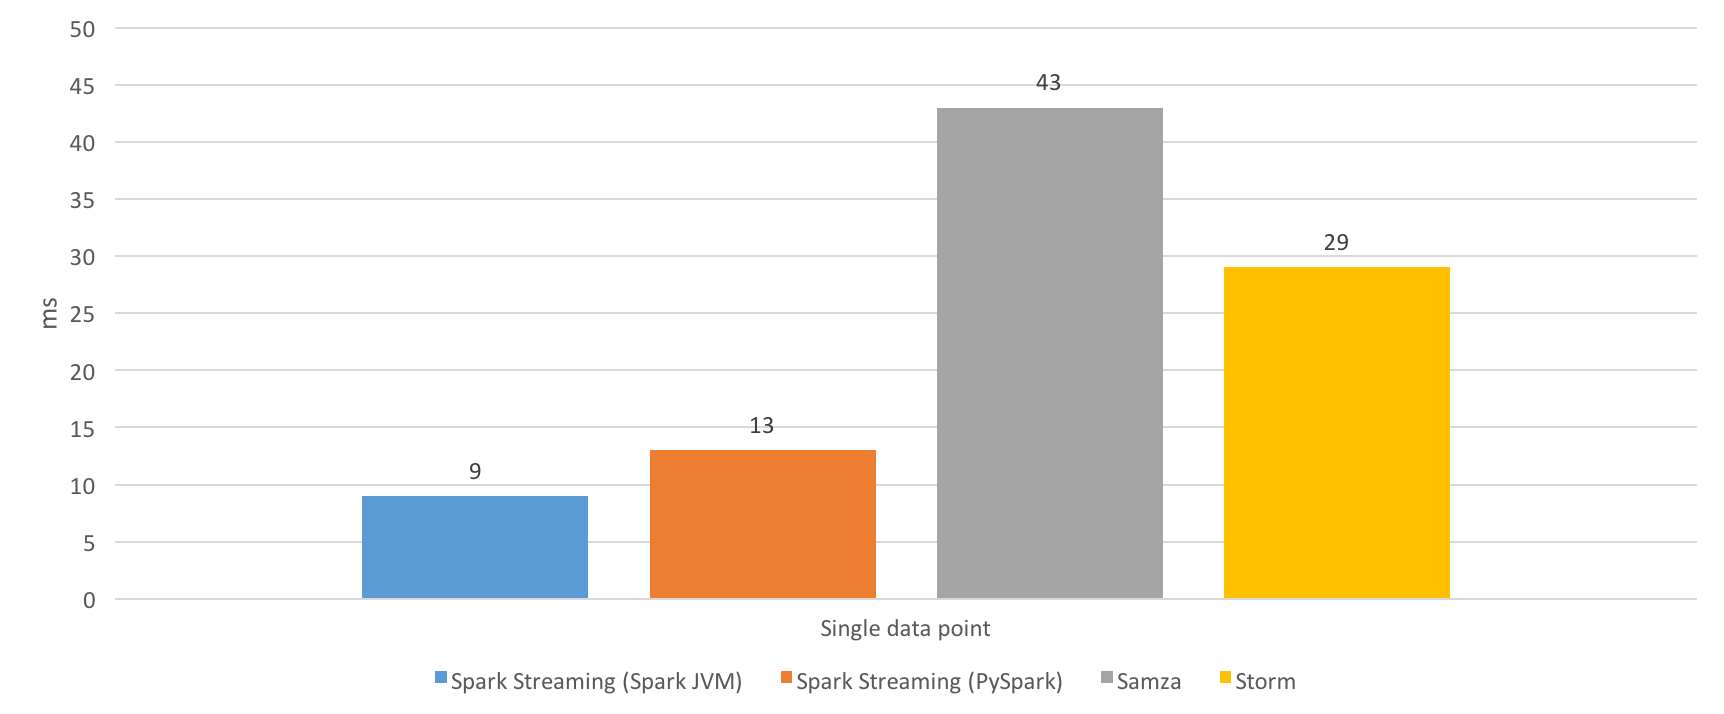
\includegraphics[width=1\textwidth]{includes/figures/fig_response_time_res}
  \caption{Results of our response time to streaming data test.}
  \label{fig:response_time_res}
\end{figure}

Essentially, what can be can be seen from these results is that both Spark Streaming APIs exhibit relatively good performance
compared to both Storm and Samza. In particular, Spark Streaming running on the Spark JVM API exhibited over $3\times$ the
performance of the next big system, Storm, and nearly $5\times$ the performance of the slowest contender, Samza. Further of
note is that at this size of data, a single sensor reading, both Spark Streaming APIs exhibit very similar performance
in relation to the other DSPS technologies.

As Spark Streaming is essentially an extension built on top of a batch processing system, the fact that it outperformed
both Samza and Storm, two technologies built from the ground up with the aim of processing data in realtime, is quite a
surprising find.

\subsubsection{Test data throughput time}

The results to the test data throughput time tests are shown in~\figref{fig:throughput_time_res}.

\begin{figure}[ht]
  \centering
  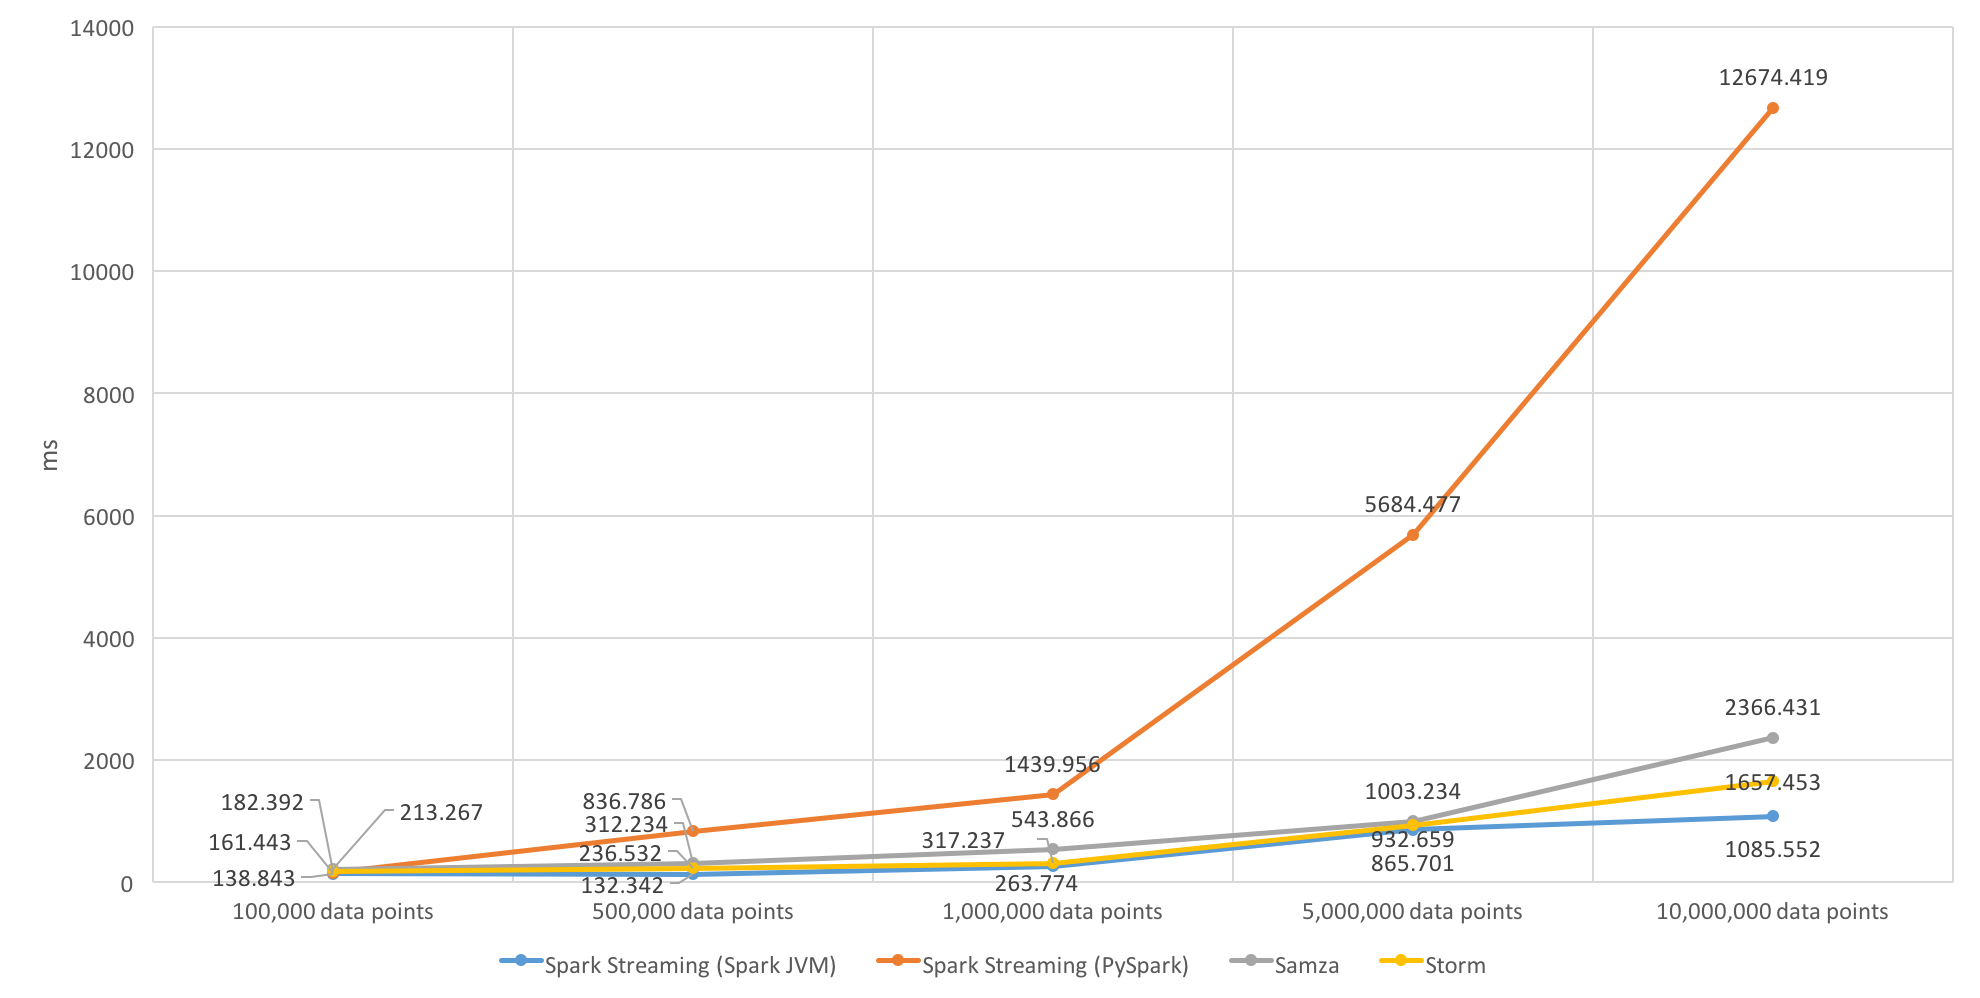
\includegraphics[width=1\textwidth]{includes/figures/fig_throughput_res}
  \caption{Results of our test data throughput time tests.}
  \label{fig:throughput_time_res}
\end{figure}

The first fact to note with these results relates to the performance of Spark Streaming, running on the PySpark API, as the
input data increases. Compared to the other technologies, Spark Streaming (PySpark) exhibits very poor scaling performance
when dealing with much larger amounts of input data, particularly with 5,\@000,\@000 data points and greater. This drop in
performance is so much of an issue that at the scale at which the results are shown, it is hard to make out differences in
performance for the other systems. Hence, to better analyse the results of the other systems, a chart from the same
data was created with the Spark Streaming (PySpark) results omitted. This can be viewed in~\figref{fig:throughput_time_res_nopyspark}.

\begin{figure}[ht]
  \centering
  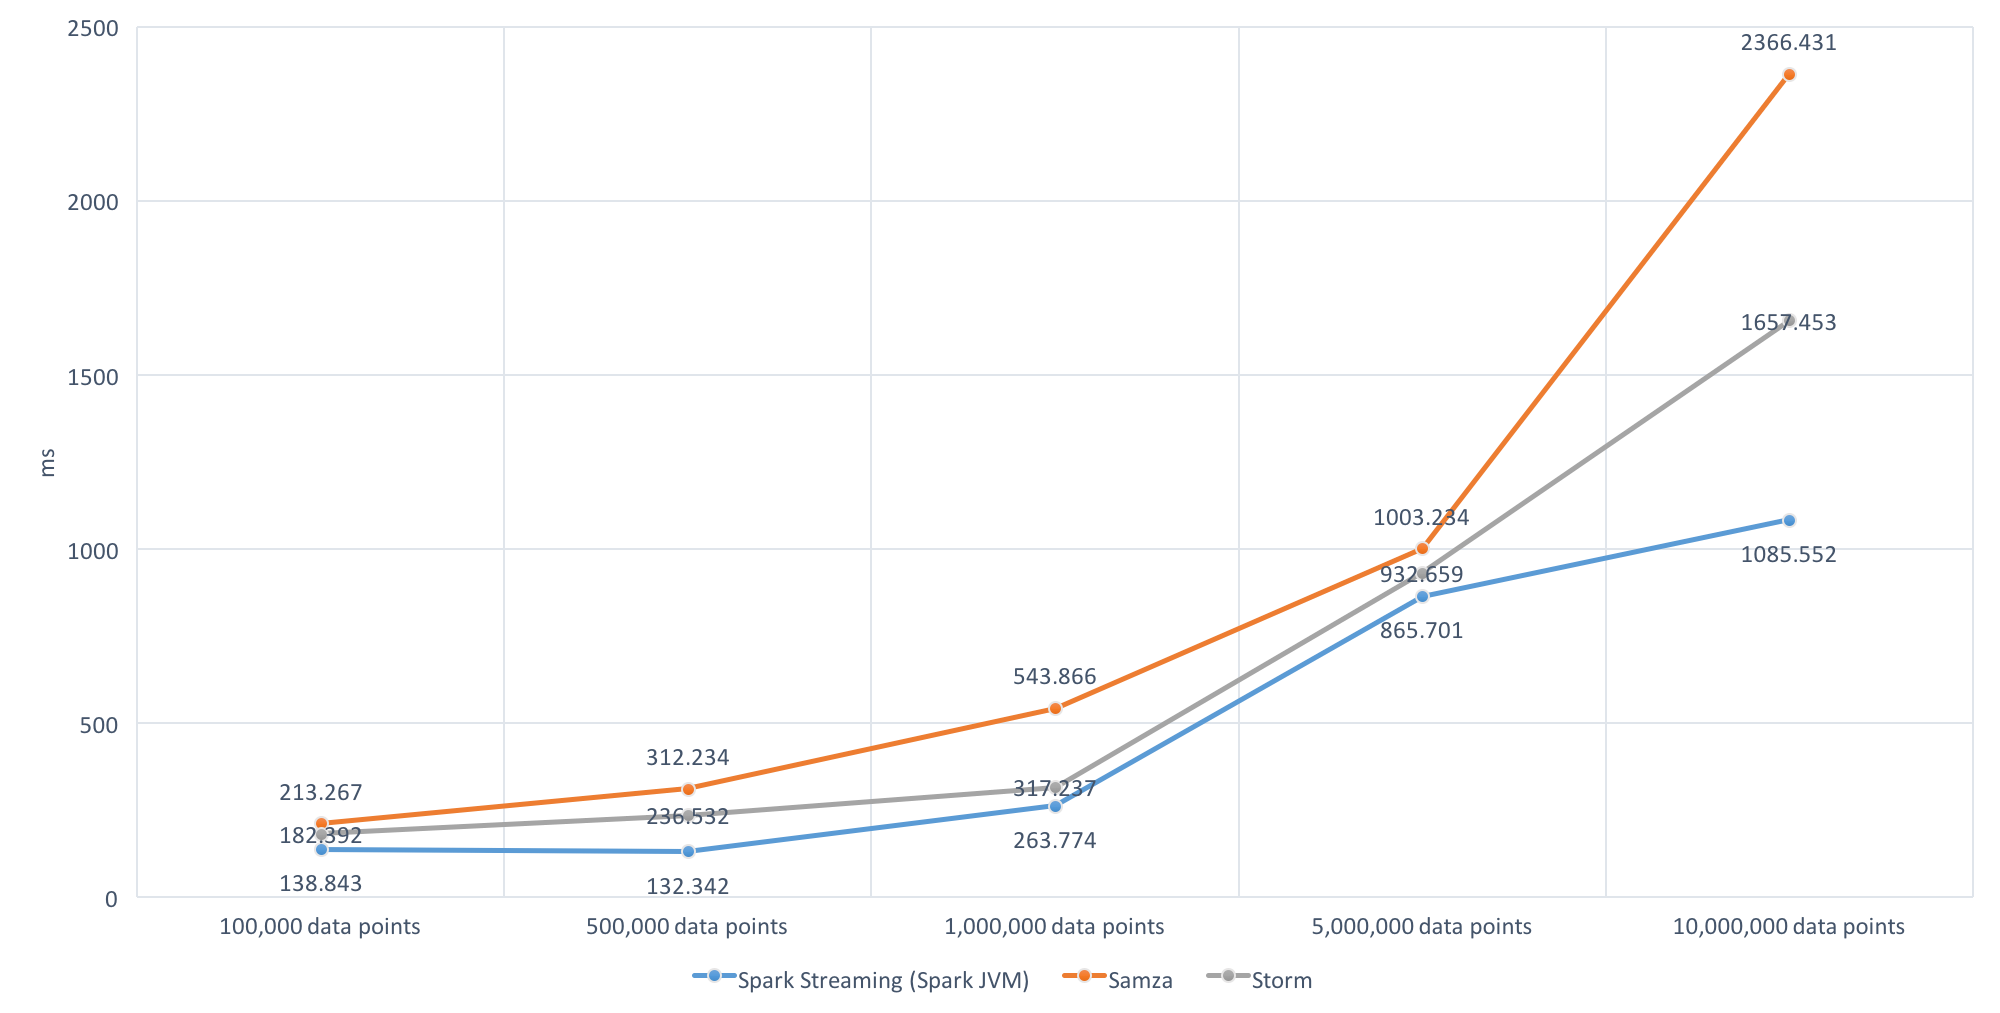
\includegraphics[width=1\textwidth]{includes/figures/fig_throughput_nopyspark_res}
  \caption{Results of our test data throughput time tests (PySpark omitted).}
  \label{fig:throughput_time_res_nopyspark}
\end{figure}

Looking the results of Spark Streaming (Spark JVM), Storm, and Samza, for the most part they show a mostly similar performance
at scale, relative to what was seen with Spark Streaming (PySpark). Spark Streaming shows the greatest performance, with
greater performance than both Storm and Samza in all tests, while Storm generally is not too far off Spark Streaming's
performance, showing a similar growth for all tests apart from the 10,\@000,\@000 data points test.

Again, Samza shows the worst overall performance out of the three candidates (not counting PySpark), with less than
half the performance of Spark Streaming on the 10,\@000,\@000 data points test.

\subsubsection{Peak system resource usage}

The results for the peak system resource usage test can be seen in~\figref{fig:resource_usage_res}.

\begin{figure}[ht]
  \centering
  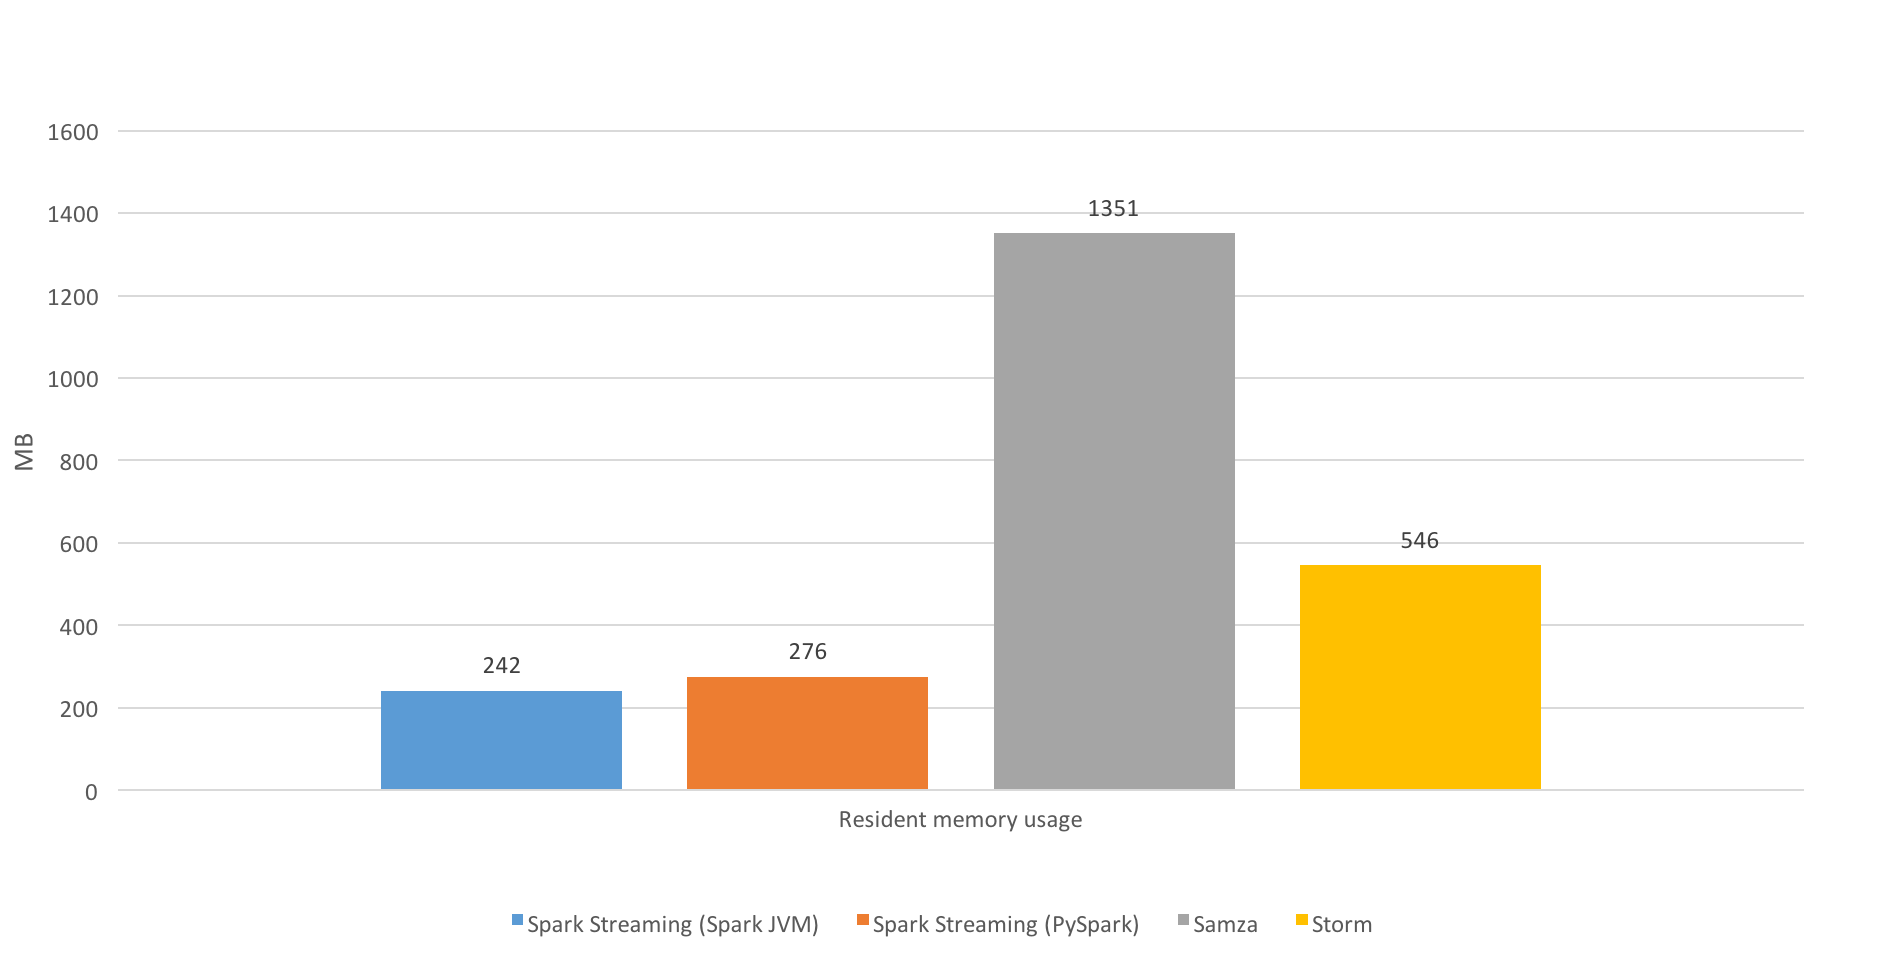
\includegraphics[width=1\textwidth]{includes/figures/fig_peak_resource_res}
  \caption{Results of our peak system resource usage test.}
  \label{fig:resource_usage_res}
\end{figure}

Interestingly, Spark Streaming excels again here, with JVM Spark having over double the performance from the next major
contender, Storm. Samza, at peak usage, takes up over $5\times$ the amount of resident memory that Spark Streaming does, and
nearly $3\times$ the amount that Storm is shown to use. A lot of this resident memory usage may be caused by a lot of the
software dependencies that Samza and Storm rely on, which Spark Streaming generally does not. Spark, the base project,
not the realtime processing extension, was designed to be an entire software ecosystem in itself, hence a lot of external
dependencies that Storm and Samza may have are not needed, possibly leading to this extreme reduction in resident memory
usage shown here.

A further point of interest here is that Spark Streaming, and thus Spark, is renowned for its in-memory computation model,
where data is placed solely in resident memory during computation. This design decision would lead to the expectation of
Spark computations using far more resident system memory than other technologies that do not make such use of resident memory.
However, as seen here, Spark Streaming is shown to use the least amount of resident memory. This may be to do with the
amounts of data used. For example, a more data-intensive workload would likely provide much higher resident system memory
usage in Spark than that of Storm or Samza.

\subsubsection{System start-up time}

The results for the system start-up time test can be seen in~\figref{fig:startup_time}.

\begin{figure}[ht]
  \centering
  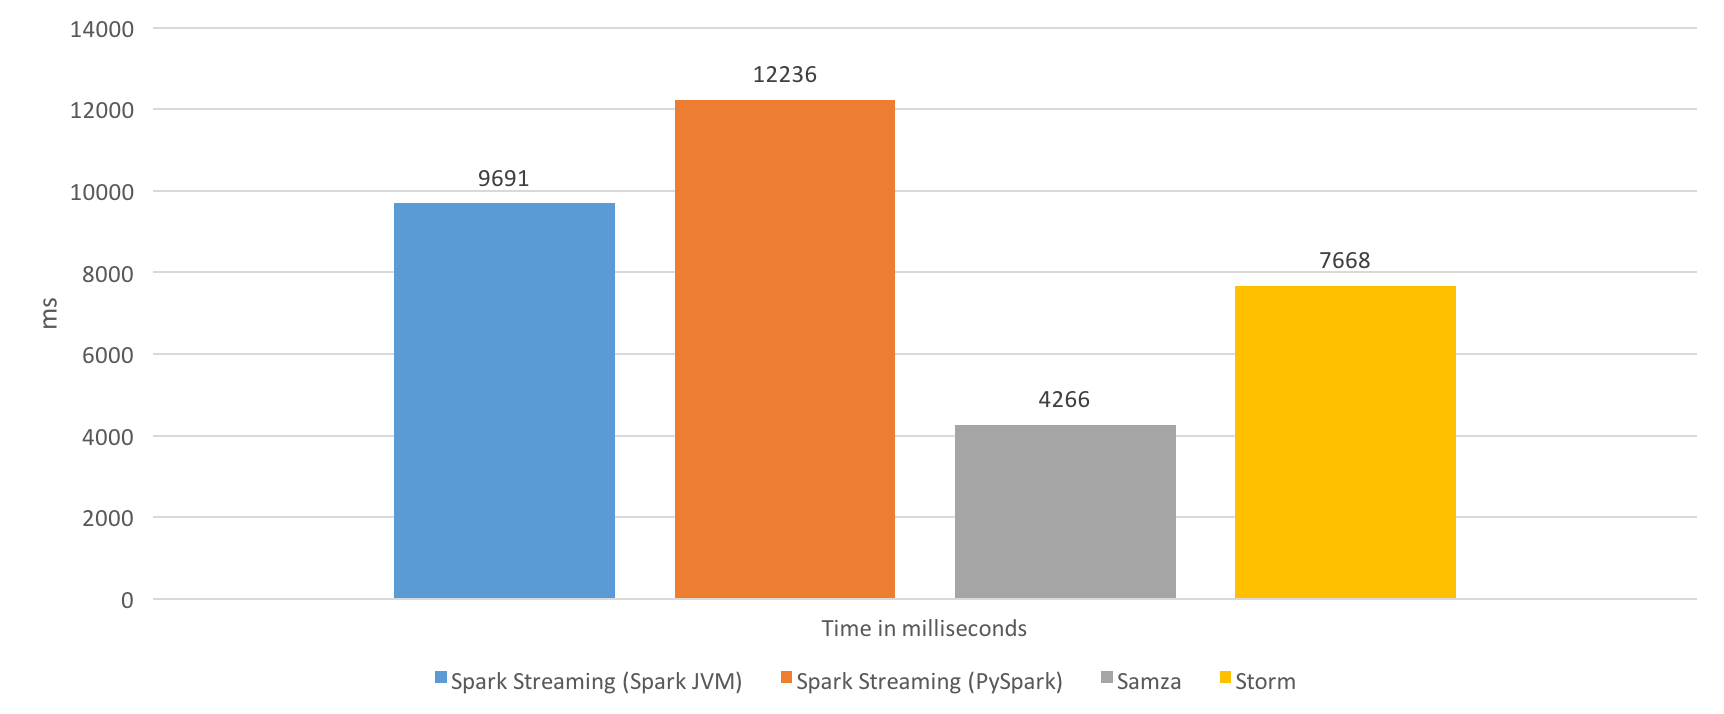
\includegraphics[width=1\textwidth]{includes/figures/fig_startup_time_res}
  \caption{Results of our system start-up time test.}
  \label{fig:startup_time}
\end{figure}

Again, we emphasise that this test is of much less importance than the previously covered quantitative tests, due to real-life usage
of the DSPS technologies. However, it is interesting of note here that Spark Streaming, the overall best performing
DSPS technology in all other performance-based tests, shows the worst performance in-terms of start-up time, particularly
the PySpark version of Spark Streaming. Samza, the overall worst performing technology, here shows the best performance,
with being able to be ready for processing from start-up in just over 4 seconds.

% subsection test_results (end)

% subsection quantitative_tests (end)


\section{Qualitative Tests} % (fold)
\label{sub:qualitative_tests}

\subsection{Tests Performed} % (fold)
\label{ssub:tests_performed}

The qualitative methods used to evaluate the candidate DSPS systems include mostly programmer-centric metrics, showing the
programming possibilities for each technology. Each of the metrics that will be compared is as follows:

\begin{itemize}
  \item Ease of extensibility
  \item Available DSPS features
  \item Ease of programmability
  \item Ease of deployment
\end{itemize}

As each of the underlying DSPS technologies are considerably different in design and usage, it is important to see how
they contrast in terms of factors that they afford.

\subsubsection{Ease of extensibility}

Ease of pipeline extensibility refers to the methods used to extend an existing pipeline, or project, existing in each
of the candidate DSPS technologies. For example, if an existing project is already in use in production, we will be measuring the
ease that each technology allows that project to be extended in the ways of adding further processing tasks to the
existing system, or restructuring an existing project processing layout (for example, a Storm topology layout). Parameters
we will be looking at include whether or not an entire project needs to be recompiled and deployed to be extended, and the
ease of modifying overall system configurations.

\subsubsection{Available DSPS features}

Available DSPS features refers to the features each candidate DSPS technology supports as they relate to Stonebraker,
\c{C}\~entintemel, and Zdonik's eight requirements for realtime data processing systems~\cite{stonebraker_8_2005}, as looked at
in the literature review chapter in~\sectref{sub:processing_conclusion}. These requirements are based on research performed
many years prior to the release of each of our candidate DSPS technologies, and most realtime data processing technologies
in general. The supported features for each technology will be compared to show the functional possibilities natively
available in each technology.

\subsubsection{Ease of programmability}

Ease of programmability refers to a number of different features including official programming language support, complexity
of required interfaces to be implemented, and complexity of required system configuration. To summarise, we will look at
the difficulty and learning-curve that may need to be overcome to program each candidate DSPS technology. Measuring this
presents a more difficult, and somewhat subjective, task compared to the metrics used in the quantitative tests, however
these will be measured using impartial comparisons of the methods which each DSPS technology affords to be programmed.

\subsubsection{Ease of deployment}

Ease of deployment refers to the methods in which each candidate DSPS technology affords its projects to be deployed and distributed.
Similar to the ease of programmability test, this metric will be measured by an impartial comparison of each possible
method of project deployment and distribution.

% subsection tests_performed (end)


\subsection{Test Results} % (fold)
\label{ssub:qual_test_results}

\subsubsection{Ease of extensibility}

Spark Streaming is noted as the worst performing technology in terms of extensibility, overall. This is mostly due to
the fact that, by design, a Spark Streaming program is generally very tightly coupled in terms of processing modules.
All processing logic revolves around the \texttt{StreamingContext} object in a Spark Streaming program, hence everything is
tightly integrated to the placement of this object. Of course, this object can be passed around different modules, however
it is a rather na\"{\i}ve solution considering the other projects exhibit loose coupling by design.

This tight coupling of logic in Spark Streaming leads to any extensions written to an existing Spark Streaming project to
be written as modifications of the original source code. This means that previously written source code need to be made
aware of the changes, and recompiled.

Likewise, in Spark Streaming, configuration is tightly coupled with the programming logic, through use of the \texttt{SparkConf}
object, on which the \texttt{StreamingContext} object is instantiated. This leads to any future changed in configuration to be
written to the original source code, thus leading to project recompilation.

Samza is noted to be far more loosely coupled than that of Spark Streaming, with any extensions of an existing project
being able to be written separately of the original code. Essentially, a Samza project's processing tasks will output
their results to specific Samza streams. On these streams, a new extension can be written to listen on, without the
existing processing tasks needing to be aware of this new extension task. This loose coupling of processing tasks is
by design in Samza, with tasks existing in a dataflow-like sequence, where tasks can be added and removed with ease.

For configuration in Samza, processing tasks and systems are configured separately to the underlying logic, using a
non-compilation necessary medium. Effectively, this means that Samza projects can be reconfigured on-the-fly without
recompilation of the entire project. This is an important factor which Spark Streaming lacks native support for.

Storm is very similar to Samza in the way that extensions can be written to extend an existing Storm topology without
modification of the existing source code being necessary. However, extensions written to an existing Storm topology do not
require knowledge of output streams from existing Storm processing tasks (bolts), which is a necessity when extending a
Samza project.

Configuration in Storm is also kept separate of the logic written in the source code, hence also does not require recompilation
to reconfigure. However, to reconfigure an existing Storm topology layout, this is generally written in source code using
the \texttt{TopologyBuilder} class, hence does require a recompilation step.

To summarise, Spark Streaming has shown to lack in extensibility, compared to the other candidate DSPS technologies, mainly
due to being tightly coupled by design, while Storm and Samza exhibit similar ease in terms of extensibility. Samza and
Storm extensions can be written separate of existing logic, without the existing logic being aware of the extensions.
This is, unfortunately, not the case with Spark Streaming.


\subsubsection{Available DSPS features}

As these features were looked at previously in the literature review chapter, in~\sectref{sub:processing_conclusion},
this table has been reconstructed in~\tabref{tab:dsps_features}, with S4 omitted due to being omitted from our candidate
DSPS systems.

\import{includes/tables/}{data_processing_compare_nos4}

One obvious point of note, at first glance of the results, is that both Spark Streaming and Samza lack many of the realtime processing
features that are present in Storm. This may be put down to the fact that both Spark Streaming, as an extension
of the greater project Spark, and Samza are still relatively immature projects. In fact, Samza only became accepted as a
top-level project at the Apache Software Foundation in January of 2015~\cite{web:apache-top-samza}, after spending years
as an Apache Incubator project. It may also be attributed to design choices of developers of both projects.

Furthermore, of note is that many features that are supported in Samza actually depend on the integration of Kafka with
Samza. If Samza is run standalone, without Kafka, certain features may not be available unless replaced with a similar
Samza-compatible pluggable system. Due to the nature of Samza and Kafka's tight coupling in most installations, a lot
of the time, the availability of these features, off-loaded to Kafka, can be taken for granted.

In relation to the IRT project, the most important features that these DSPS systems support are arguably \textbf{SQL on
streams} and \textbf{Stored and streaming data}. These features refer to the possibility of running more traditional
batch processing functions, such as aggregate functions like map reduce, on the data streams that are being processed
otherwise in realtime. As the IRT project at current uses a lot of batch processing applied to their data, it would be
much more ideal if the DSPS technology to be used also had the possibility of affording this type of processing in
conjunction with realtime processing.

From the results, it is shown that both Storm and Spark afford these features.
Storm, via the Trident extension, allows both batched data processing through aggregate functions, and an SQL-like query
language~\cite{web:storm-trident}. Spark Streaming, being built on top of the batch processing project, Spark, natively
supports batch processing by off-loading to Spark, and an SQL-like query language through the new Spark SQL extension~\cite{web:sparksql}.
Conversely, Samza does not afford any native type of batch processing functionality, or any SQL-like query language at
the time of writing.


\subsubsection{Ease of programmability}

Spark Streaming has been noted as being the most accessible of the candidate DSPS technologies in terms of programmability.
Spark Streaming, as of version 1.2.0, has official support for Java, Scala, and Python (however some of the functionality deemed
less important is yet to be implemented in the Python API). Storm has native support for Java and Clojure, and essentially
any programming language through use of a Thrift definition file\footnote{https://thrift.apache.org/}, however official
documentation is only provided for Java and Clojure. Samza only has native support for Java.

Writing Spark Streaming projects, and also Storm and Samza projects,
in JVM languages of course require compilation to JVM bytecode before they are to be run, and also having the requirement
that the compiled bytecode be packaged as a distributable JAR archive. Python use with PySpark, being an
interpreted language, allows for Spark Streaming projects to be written and run directly from the Python source files
deployed to a Spark installation. This has been noted to greatly ease the aspect of getting a new Spark Streaming project
up and running, without many compilation and assembly steps that are required in the JVM language DSPS technologies.

Storm and Samza have been noted as having a far higher learning curve to that of Spark Streaming, due to the number of
interfaces which are required to be implemented to make even the most simple of projects, and the required configuration
that is necessary for the project to run properly. Spark Streaming does away with these interfaces, and instead all processing
logic surrounds the \texttt{StreamingContext} class, meaning that as long as this class is instantiated, all the possible processing
functions are available to be used. Thus, a simple processing pipeline based on simple processing logic implemented in each
system would require a number of different files, each implementing required interfaces, in Storm and Samza, while the
same logic in Spark Streaming could be done in a number of lines in any supported programming language.

Samza, in particular, has been noted as having the most steep of the learning curves, in terms of programmability, due
to a required knowledge of many of the underlying software dependencies, such as Kafka, ZooKeeper, and various serialisers
and deserialisers for Samza messages. Required configuration of a Samza project requires an understanding of these systems for
even the most simple of processing tasks, while most of the underlying systems in Storm and Spark Streaming are abstracted
away from the programmer, who generally does not need to worry about these unless performing more advanced tasks.

In terms of required configuration, Spark Streaming allows for the most ease in configuring, due to a low level understanding
of Spark configuration not being needed for most tasks. Storm also has somewhat of a easy required configuration knowledge,
mostly due to having the more complicated configuration options being abstracted away from the programmer unless necessary, and the
majority of configuration being defined in the topology file. Samza, however, requires separate, and particularly verbose,
configuration files for every task and system within a Samza project, as well as many configuration options not having
defaults. Again, this leads to a good understanding of Samza being needed to configure even a simple project, and a lot
of configuration to be thought about, particularly if a Samza system expands to be greater than a small number of different
processing tasks.

In summary, Spark Streaming has been noted as the most simple of the candidate DSPS technologies in terms of programmability
and overall learning curve. Simple projects are able to be configured and written in a small amount of lines of code.
Storm presents the next most simple technology with a lot of the configuration and software dependencies being abstracted
away from the programmer. Samza comes in last, with the largest learning curve, due to a good understanding of the overall
Samza project, along with Samza software dependencies needed to implement even a simple Samza project.


\subsubsection{Ease of deployment}

Projects written for each of the DSPS technologies are expected to be deployed and distributed in similar ways. As each
of the technologies are built on JVM technologies, they require compiled JVM bytecode to be packaged as a JAR file, generally
using a build automation tool, such as Maven\footnote{https://maven.apache.org/} or Gradle\footnote{https://gradle.org/}.
However, for deployment and distribution of Spark Streaming projects written in Python, these compilation and build
assembly steps are not necessary, with Python and Scala Spark Streaming projects affording deployment simply as the Python
or Scala source files themselves. This greatly eases overall deployment, and distribution of Spark Streaming projects between
different Spark Streaming installations residing on different clusters.

Furthermore, Storm and Samza require the set-up of external technology dependencies, such as Kafka or ZooKeeper, on the
cluster on which they will be run, if the implemented project requires such dependencies. Spark Streaming can be deployed
without external technology dependencies as the Spark project provides Spark distributions with all such dependencies built-in
and pre-configured~\cite{web:spark-downloads}.

% subsection test_results (end)

% subsection qualitative_evaluations (end)


\section{Discussion} % (fold)
\label{sub:eval_discussion}

Looking over the results of both the quantitative performance-based results, and the qualitative feature-based results,
a few points are of note in regards to each of the candidate DSPS technologies. First, Spark Streaming has shown the
overall greatest performance while managing to have the lowest resident memory footprint. Both the Spark JVM and PySpark
based Spark Streaming versions show great performance, however the Spark JVM version shows the best performance overall
given that the PySpark version does not scale well when dealing with larger amounts of data being streamed in.
Spark Streaming also showed the lowest learning curve and was the overall easiest technology to write realtime processing
logic in.

However, while Spark Streaming has been shown to have the greatest performance through the results of the quantitative
tests, it very much falls short in relation to ease of extensibility due to the tightly coupled nature of Spark Streaming
projects. As all realtime processing logic is focused around a single class which affords the DStream functionality,
any extensions written to alter an existing project require the modification of the original project, tightly integrating the
extension logic into the existing logic.

Storm, on the other hand, showed the next best performance and resident memory footprint after Spark Streaming, through
the results of the quantitative tests. The performance of Storm has been shown to be closer to that of Spark Streaming,
JVM version, rather than that of Samza. Furthermore, Storm affords the next best option in terms of learning curve and
ease of writing realtime processing logic to that of Spark Streaming, and it has shown to be a much more mature project
to Samza, with a lot more available documentation.

Samza has shown to perform badly in almost all the tests, both qualitative and quantitative, apart from ease of extensibility where it beat Spark Streaming.
This is an unfortunate result from the most immature of all the candidate DSPS technologies, however it is not an overly
surprising outcome.

% subsection discussion (end)


\section{DSPS Technology Recommendations} % (fold)
\label{sub:dsps_technology_recommendations}

As discussed, while Spark Streaming has been shown to have the overall greatest performance of the three candidate DSPS
technologies, due to its failing, in terms of extensibility, we cannot recommend it for use in the Monash University IRT
project. This stems back to our third research question for this project, looking at the possibility of extending projects
developed in each of the candidate DSPS technologies.

As Storm has shown the second best performance to Spark Streaming, the second best outcome in most qualitative tests,
and shown to be the overall most extensible of the three technologies, it is a much better contender for use in the Monash
University IRT project.

We cannot recommend the use of Samza, in light of its performance in relation to the other two technologies in all tests.
Both of the other candidate technologies provide better outcomes overall in most areas.

Hence, we are recommending the use of Storm in the Monash University IRT project. We believe that it exhibits all the
characteristics required for a DSPS technology in the IRT project, and exhibits relatively positive performance. It affords
use in an advanced project, subject to many changes, such as the IRT project, and it is
also the most mature of the three candidate technologies, allowing for much documentation and support available to be found on the
Internet.

Spark Streaming is our runner-up recommendation, showing great performance, and a low learning curve. We recommend
Spark Streaming to be used in simple realtime processing projects, where change and extension may be unnecessary or not
required often.

% subsection dsps_technology_recommendations (end)


\section{Conclusion} % (fold)
\label{sub:evaluation_conclusion}

In conclusion, we have nominated Storm as our recommended data stream processing system technology for use in the Monash
University Institute of Railway Technology project. Overall, we have shown it to exhibit great performance and features
in terms of programmability and extensibility. It has shown to have a steeper learning curve to that of Spark Streaming,
however Spark Streaming has shown to be a less viable option for large, and constantly changing projects, such as the IRT
project.

This nomination as our recommended DSPS technology comes after performing many suitable tests, using both quantitative performance-based
metrics and qualitative use-based metrics, and evaluating it in comparison to our other candidate DSPS technologies, Samza and Spark Streaming.


% subsection conclusion (end)
